\documentclass{article}
\usepackage[utf8]{inputenc}
\usepackage[left=2.5cm, top=2.5cm, right=2.5cm, bottom=2.5cm]{geometry}
\usepackage[spanish]{babel}
\usepackage{hyperref}
\usepackage{graphicx}
\usepackage{float}
\usepackage{listings}
\usepackage{xcolor}

\setlength{\parskip}{10pt}
\definecolor{vscdbg}{rgb}{0.80,0.80,0.85}      % Slightly darker Background
\definecolor{vscdstring}{rgb}{0.13,0.55,0.13}  % Strings (green)
\definecolor{vscdcomment}{rgb}{0.46,0.54,0.60} % Comments
\definecolor{vscdkeyword}{rgb}{0.56,0.38,0.68} % Keywords (darker for contrast)
\definecolor{vscdnumber}{rgb}{0.48,0.38,0.26}  % Numbers (darker for contrast)
\definecolor{vscdgray}{rgb}{0.40,0.40,0.40}    % Line numbers
\definecolor{vscdtext}{rgb}{0.30,0.30,0.30}    % Main text (lighter gray)
\lstdefinestyle{mystyle}{
    backgroundcolor=\color{vscdbg},
    basicstyle=\ttfamily\footnotesize\color{vscdtext},
    commentstyle=\color{vscdcomment}\itshape,
    numberstyle=\tiny\color{vscdgray},
    stringstyle=\color{vscdstring},
    breakatwhitespace=false,
    captionpos=b,
    numbers=left,
    showspaces=false,
    showstringspaces=false,
    showtabs=false,
    xleftmargin=50pt,
    xrightmargin=50pt,
    frame=single,
    aboveskip=10pt,
    belowskip=10pt,
    columns=flexible
}

\lstset{style=mystyle}

\definecolor{consolebg}{rgb}{0.95,0.95,0.92}
\definecolor{consoletext}{rgb}{0.20,0.20,0.20}
\definecolor{consoleprompt}{rgb}{0.60,0.60,0.60}
\lstdefinestyle{console}{
    backgroundcolor=\color{consolebg},
    basicstyle=\ttfamily\footnotesize\color{consoletext},
    numberstyle=\tiny\color{consoleprompt},
    commentstyle=\color{consoleprompt}\itshape,
    showstringspaces=false,
    showspaces=false,
    showtabs=false,
    frame=single,
    xleftmargin=30pt,
    xrightmargin=30pt,
    aboveskip=8pt,
    belowskip=8pt,
    columns=flexible,
    numbers=none,
    keywordstyle=\color{consoleprompt},
    moredelim=**[is][\color{consoleprompt}]{@}{@}
}

\linespread{1}
\hypersetup{
    pdftitle={(TA047) Trabajo Práctico 1},
    pdfauthor={Patricio Ibar - 109569},
    pdfsubject={Informe del Trabajo Práctico 1 de la materia Ciencia de Datos TA047},
}
\title{
    
\includegraphics[width=0.5\textwidth]
    {imagenes/Logo-fiuba.png}

    \vspace{1cm}
    \textbf{(TA047) - Ciencia de Datos} \\
    \vspace{1cm}
    \textbf{Trabajo Práctico 1 (2C2025)}
}
\author{Patricio Ibar - Padrón 109569}
\date{11 de septiembre de 2025}

\begin{document}
    
    \maketitle
    \newpage

    \tableofcontents
    \newpage

    \section{Introducción}
En el presente informe se documentan los pasos seguidos para la realización del Trabajo Práctico 1 de la materia Ciencia de Datos (TA047) de la Facultad de Ingeniería de la Universidad de Buenos Aires. El objetivo del trabajo práctico es realizar un análisis exploratorio de conjunto de datos. El análisis incluye la limpieza y preparación de los datos, la realización de consultas y visualizaciones, y la interpretación de los resultados obtenidos. La consigna del trabajo práctico y los datos a analizar pueden encontrarse en el siguiente enlace: \url{https://organizacion-de-datos-7506-argerich.github.io/consigna_tp1_2c2025.html}.

Se trabajó utilizando Python y la librería pandas para la manipulación y análisis de datos. Además, se utilizaron otras librerías como matplotlib y seaborn para la visualización de datos.

Tanto el código fuente, junto con las visualizaciones, como el informe se encuentran disponibles en el siguiente repositorio de GitHub: \url{https://github.com/patricioibar/datos-tp1}

    \section{Limpieza de Datos}
\label{sec:limpieza_de_datos}

Luego de cargar los datos y previo a la realización de análisis exploratorios, es fundamental llevar a cabo un proceso de limpieza y preparación de los datos.
En esta sección se describen los pasos realizados para la limpieza y preparación de los datos antes de su análisis. Se detallan las técnicas utilizadas para manejar valores faltantes, reducción del uso de memoria y la transformación de variables.

\subsection{Carga de Datos}

Los datos fueron cargados desde un archivo CSV utilizando la librería pandas de Python. Al cargar una tabla, se especificaron las columnas a utilizar para reducir el uso de memoria. También se especificaron los tipos de datos para cada columna para asegurar una correcta interpretación. Especificar el tipo de datos también optimiza el uso de memoria, ya que pandas asigna el tipo de datos más eficiente posible.

Los tipos de datos utilizados fueron:
\begin{itemize}
    \item \texttt{uint32} para identificadores y cantidades.
    \item \texttt{float32} para precios y totales.
    \item \texttt{category} para columnas con un número limitado de valores únicos, como estados o método de pago.
    \item \texttt{datetime64} para fechas y horas.
    \item \texttt{string} para texto sin formato.
    \item \texttt{bool} para valores booleanos.
\end{itemize}

Todas estas acciones se realizan a través de la función \texttt{pd.read\_csv()} de pandas, que permite especificar las columnas a cargar y sus tipos de datos. A continuación se muestra un ejemplo de cómo se realiza la carga de datos:

\begin{figure}[H]
\begin{lstlisting}[language=Python, xleftmargin=70pt, xrightmargin=70pt]
# Carga de la tabla de ordenes para las consultas propuestas por el enunciado
orders = pd.read_csv(
    'data/orders.csv',
    usecols=[
        'order_id',
        'customer_id',
        'status',
        'payment_method',
        'billing_address',
        'discount_amount'
    ],
    dtype={
        'order_id': 'uint32',
        'customer_id': 'uint32',
        'status': 'category',
        'discount_amount': 'float32',
        'payment_method': 'category'
    },
)
\end{lstlisting}
\end{figure}

\subsection{Manejo de Valores Faltantes}

Es común encontrar valores faltantes en los conjuntos de datos. Estos valores pueden ser el resultado de errores en la recolección de datos o simplemente porque la información no estaba disponible en el momento de la recolección. Por ejemplo, para las primeras consultas del enunciado, se identificaron valores faltantes en las columnas \texttt{status} y \texttt{billing\_address}.
La presencia de valores faltantes puede ocasionar problemas al ejecutar ciertas operaciones o análisis, por lo que es crucial abordarlos adecuadamente.
Además, es importante manejar los valores faltantes de una forma acorde al análisis que se desea realizar. En algunos casos puede ser necesario eliminar filas o columnas con valores faltantes, mientras que en otros casos puede ser más apropiado darle un valor específico.

Por ejemplo, tanto en las columnas \texttt{status} como en \texttt{billing\_address}, se decidió dar un valor por defecto a los valores faltantes. Para esto se utilizó la función \texttt{fillna()} de pandas, que permite reemplazar los valores faltantes con un valor específico. En este caso, se decidió reemplazar los valores faltantes con el valor \texttt{"UNDEFINED"}.

\subsection{Normalización de Datos}

En muchos casos pueden encontrarse diferentes valores en una misma columna que representan la misma información. Por ejemplo, en la columna \texttt{status} pueden encontrarse los valores \texttt{"delivered"}, \texttt{"DELIVERED"} y \texttt{"Delivered"}, que representan el mismo estado de una orden. Para evitar confusiones y facilitar el análisis, es importante normalizar estos valores a un formato consistente.

La estrategia que adopté fue convertir todos los valores a mayúsculas utilizando la función \texttt{Series.str.upper()} de pandas, además de quitar los posibles espacios que el valor pueda tener al comienzo y al final, utilizando la función \texttt{Series.str.strip()}. \\
Luego de realizar estas `normalizaciones', si la columna es categórica, es importante reconvertirla al tipo de dato \texttt{category} para optimizar el uso de memoria.

    \section{Características del Dataset}

El dataset provisto por la cátedra contiene información sobre órdenes de compra, clientes, categorías, productos y reseñas de lo que podría ser una tienda en línea. \\
Al hacer varias consultas y visualizar los resultados se puede deducir que los datos no son reales, sino que son simulados. 
Por ejemplo, los nombres y apellidos de los clientes son muy genéricos y repetitivos, los nombres de los productos parecen ser palabras aleatorias sin significado, las ciudades tienen nombres inventados, las direcciones tienen estados y códigos postales de Estados Unidos pero países diferentes, etc. También aparecen valores sin sentido para algunos motivos de movimiento de inventario, como por ejemplo `Theft' o `Damage', pueden aparecer con valores positivos o negativos, lo carece de sentido real.

Además de esto, al realizar las consultas se encuentra con que los resultados son considerablemente uniformes, lo que refuerza la idea de que los datos son simulados. Esto es una lástima, pues dificulta la realización de análisis más profundos y la obtención de conclusiones interesantes.

A continuación muestro algunos gráficos que ilustran estas características simuladas o uniformes para las tablas \texttt{orders}, \texttt{customers} e \texttt{inventory\_logs}. Todas las consultas y gráficos de esta sección pueden encontrarse en el notebook \href{https://github.com/patricioibar/datos-tp1/blob/main/datos_uniformes.ipynb}{\texttt{datos\_uniformes.ipynb}}.

\subsection{Usuarios}
Para empezar, podemos ver en la figura \ref{fig:usuarios_por_pais} la cantidad de usuarios por país. Se puede observar que en todos los paises hay una cantidad muy similar de usuarios, y aún más, hay una cantidad también similar de usuarios sin país determinado. Esto es poco realista, ya que en la vida real la distribución de usuarios por país suele ser muy desigual debido a cuestiones socioeconómicas o poblacionales.
\begin{figure}[H]
    \centering
    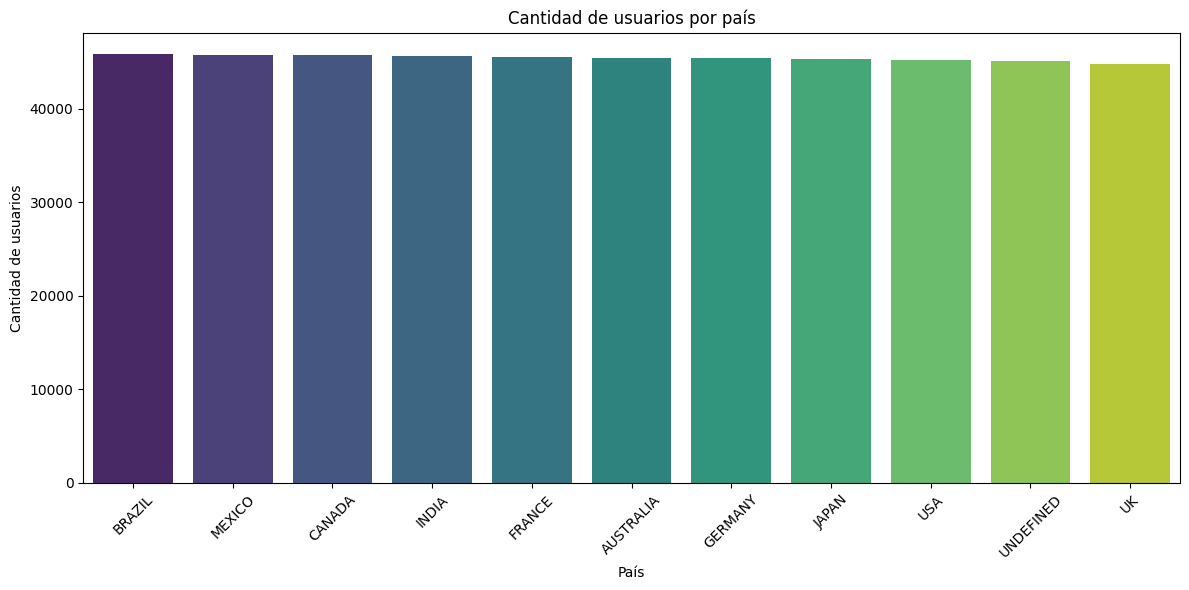
\includegraphics[width=0.8\textwidth]{imagenes/datos_uniformes/usuarios_por_pais.png}
    \caption{Cantidad de usuarios por país}
    \label{fig:usuarios_por_pais}
\end{figure}

En las siguientes dos figuras, podemos ver ilustrados los nuevos usuarios que se registran cada mes, diferenciados según el segmento al que pertenecen.
En estos gráficos se puede observar que, si bien no hay una cantidad exactamente igual de usuarios nuevos cada mes, la diferencia es muy pequeña. La mayor diferencia de nuevos usuarios está en el primer mes y el último mes registrado (ver figura \ref{fig:usuarios_nuevos_por_segmento_y_mes_de_registro}), sin embargo la proporción de nuevos usuarios respecto al total de usuarios sigue siendo muy similar en todos los meses (ver figura \ref{fig:proporcion_de_nuevos_usuarios}).

Otra cosa que se puede observar en estos gráficos es que la mayoría de los usuarios pertenecen al segmento \texttt{Regular}, mientras que los segmentos \texttt{Premium} y \texttt{Budget} son tienen menor volumen. Aún así, es destacable la proporción casi idéntica en estos últimos dos segmentos.

\begin{figure}[H]
    \centering
    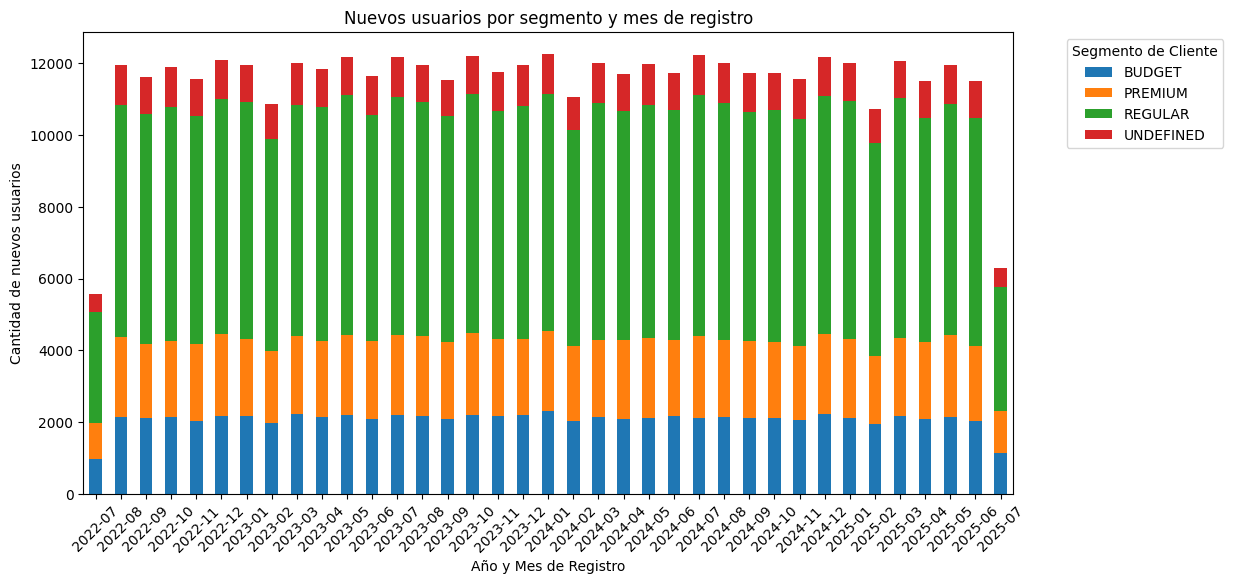
\includegraphics[width=0.8\textwidth]{imagenes/datos_uniformes/usuarios_nuevos_por_segmento_y_mes_de_registro.png}
    \caption{Cantidad de usuarios nuevos por segmento y mes de registro}
    \label{fig:usuarios_nuevos_por_segmento_y_mes_de_registro}
\end{figure}
\begin{figure}[H]
    \centering
    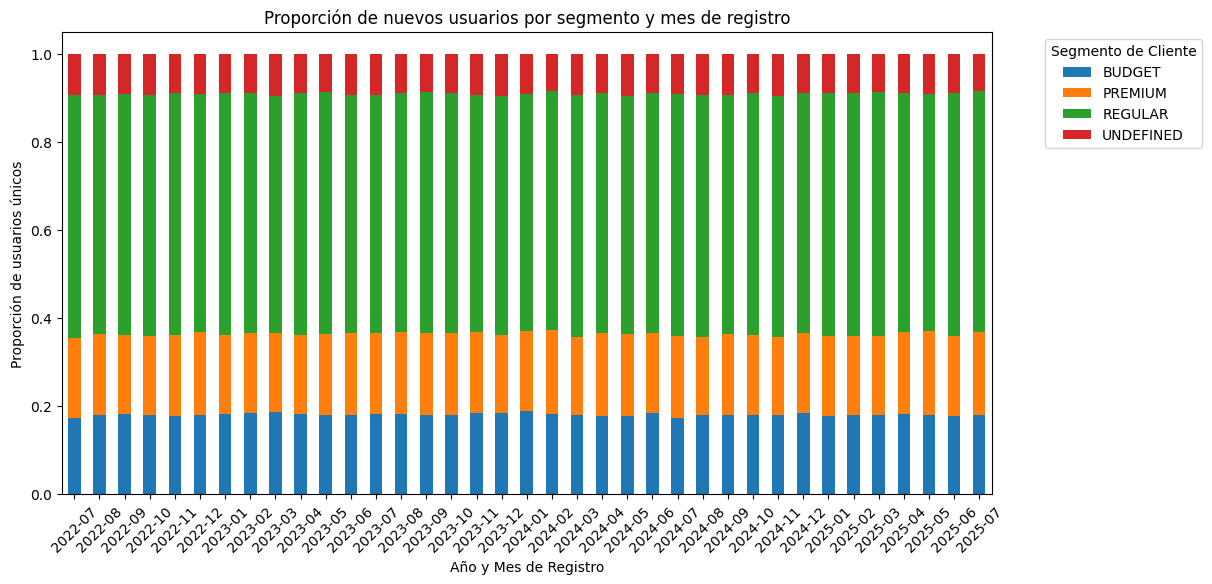
\includegraphics[width=0.8\textwidth]{imagenes/datos_uniformes/proporcion_de_nuevos_usuarios.png}
    \caption{Proporción de nuevos usuarios por segmento y mes de registro}
    \label{fig:proporcion_de_nuevos_usuarios}
\end{figure}

A continuación se muestran dos gráficos que ilustran la cantidad de usuarios por estado. En la figura \ref{fig:usuarios_por_estado} se puede observar que la mayoría de los estados tienen una cantidad similar de usuarios. En esta primera figura se visualiza una escala de 0 a 7000, y vemos que todos los estados tienen colores muy similares.

\begin{figure}[H]
    \centering
    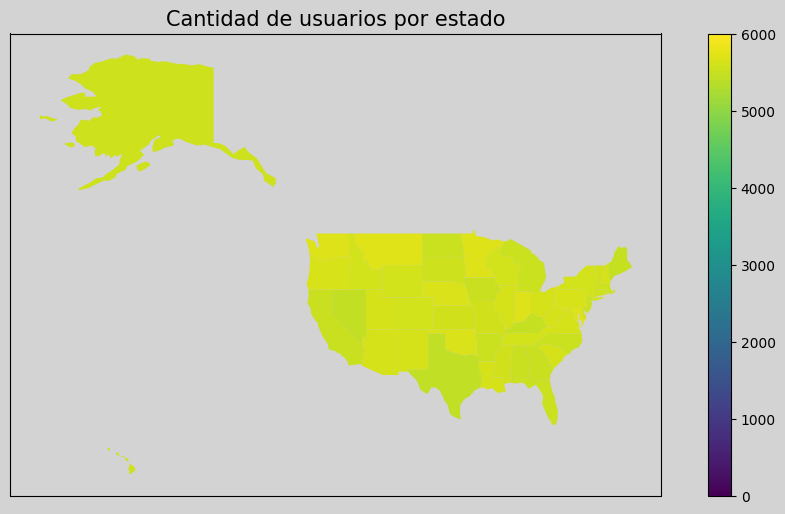
\includegraphics[width=0.8\textwidth]{imagenes/datos_uniformes/usuarios_por_estado.png}
    \caption{Cantidad de usuarios por estado}
    \label{fig:usuarios_por_estado}
\end{figure}

En la figura \ref{fig:usuarios_por_estado_closer} se puede ver el mismo mapa con una escala más cerrada, aproximadamente de 6300 a 6700. En este gráfico sí se pueden notar colores más variados. Aún así hay que notar que la diferencia entre el estado con más usuarios y el estado con menos usuarios es de a lo sumo 400 usuarios, lo cual es una diferencia bastante baja tomando en consideración el total de usuarios por estado. Esto refuerza la idea de que los datos son simulados y no representan una distribución realista de usuarios por estado. Notar como, por ejemplo, el estado de Alaska  tiene muchos más usuarios que Texas, lo cual es muy improbable en un escenario real.

\begin{figure}[H]
    \centering
    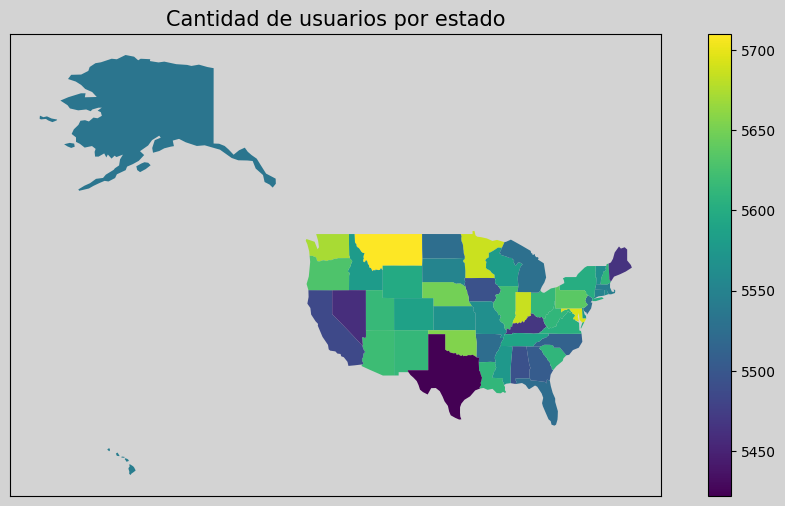
\includegraphics[width=0.8\textwidth]{imagenes/datos_uniformes/usuarios_por_estado_closer.png}
    \caption{Cantidad de usuarios por estado (detalle)}
    \label{fig:usuarios_por_estado_closer}
\end{figure}

\subsection{Órdenes}

En la figura \ref{fig:ordenes_por_estado} se pueden visualizar la cantidad de órdenes totales por estado. Nuevamente, se puede observar que la mayoría de los estados tienen una cantidad similar de órdenes, a excepción de los estados militares de Estados Unidos (AA, AE, AP) que tienen una cantidad considerablemente mayor de órdenes, casi exactamente el doble.

\begin{figure}[H]
    \centering
    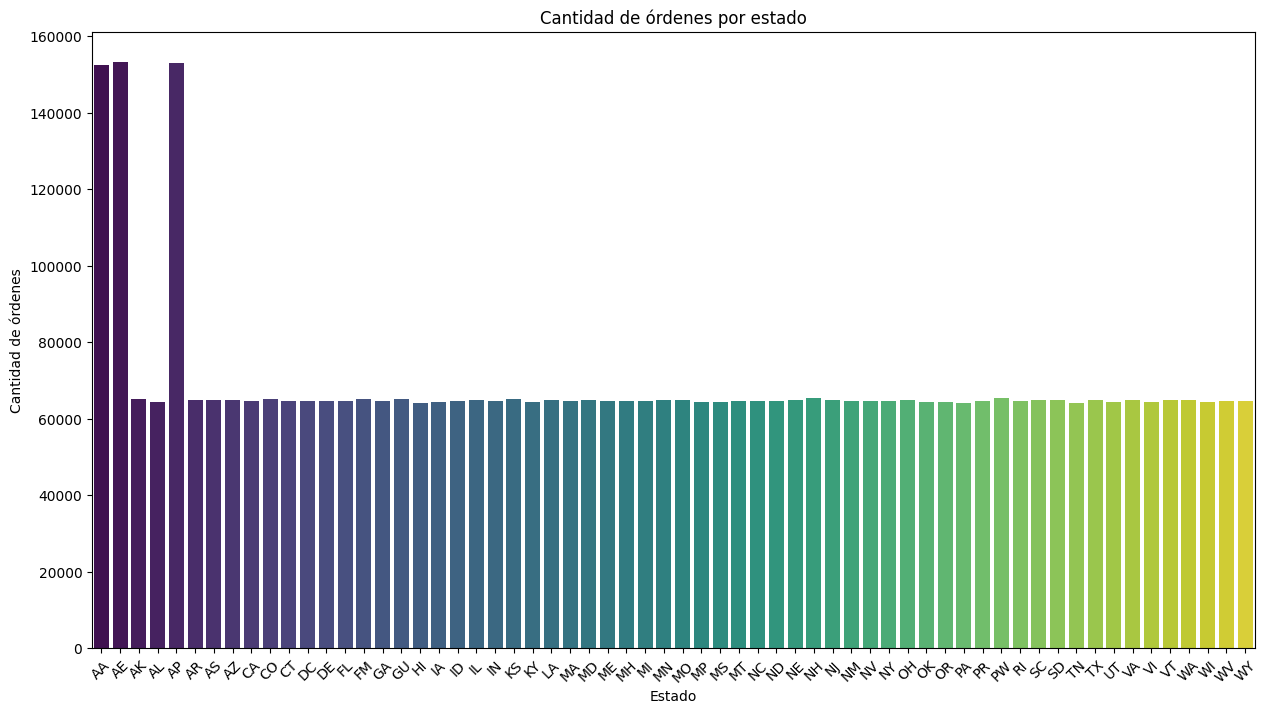
\includegraphics[width=0.8\textwidth]{imagenes/datos_uniformes/ordenes_por_estado.png}
    \caption{Cantidad de órdenes por estado}
    \label{fig:ordenes_por_estado}
\end{figure}

\begin{figure}[H]
    \centering
    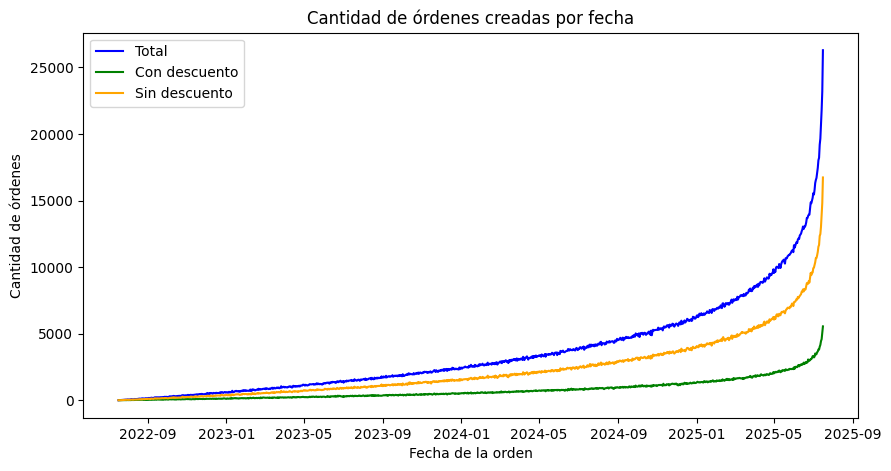
\includegraphics[width=0.8\textwidth]{imagenes/datos_uniformes/cantidad_de_ordenes_por_fecha.png}
    \caption{Cantidad de órdenes por fecha (agrupados con descuento, sin descuento y totales)}
    \label{fig:cantidad_de_ordenes_por_fecha}
\end{figure}

En la figura \ref{fig:cantidad_de_ordenes_por_fecha} se puede observar la cantidad de órdenes por fecha (i.e. la cantidad de filas en la tabla \texttt{orders} por fecha), diferenciados para órdenes con descuento, sin descuento y el total. Se puede observar que las tres curvas siguen una tendencia muy marcada, parecida a una curva exponencial, con desviaciones muy pequeñas. \\
Esto nos da una idea de cómo se pueden haber simulado los datos, podemos inferir que se utilizó algún tipo de función matemática para generar estas cifras y que se utilizó un porcentaje fijo de órdenes con descuento respecto al total de órdenes.

En la figura \ref{fig:ordenes_por_estado_en_el_tiempo} se puede observar la proporción de órdenes por estado en el tiempo. Cada color representa uno de los estados. Se puede observar nuevamente la tendencia muy marcada en todos los estados, con desviaciones muy pequeñas. Se puede apreciar muy bien cómo la cantidad de órdenes por mes es casi idéntica para todos los estados. La única excepción son las cantidades en los estados militares como se vió en la figura \ref{fig:ordenes_por_estado}, que aún puede verse que tienen que siguen una tendencia similar a la de los demás estados.

\begin{figure}[H]
    \centering
    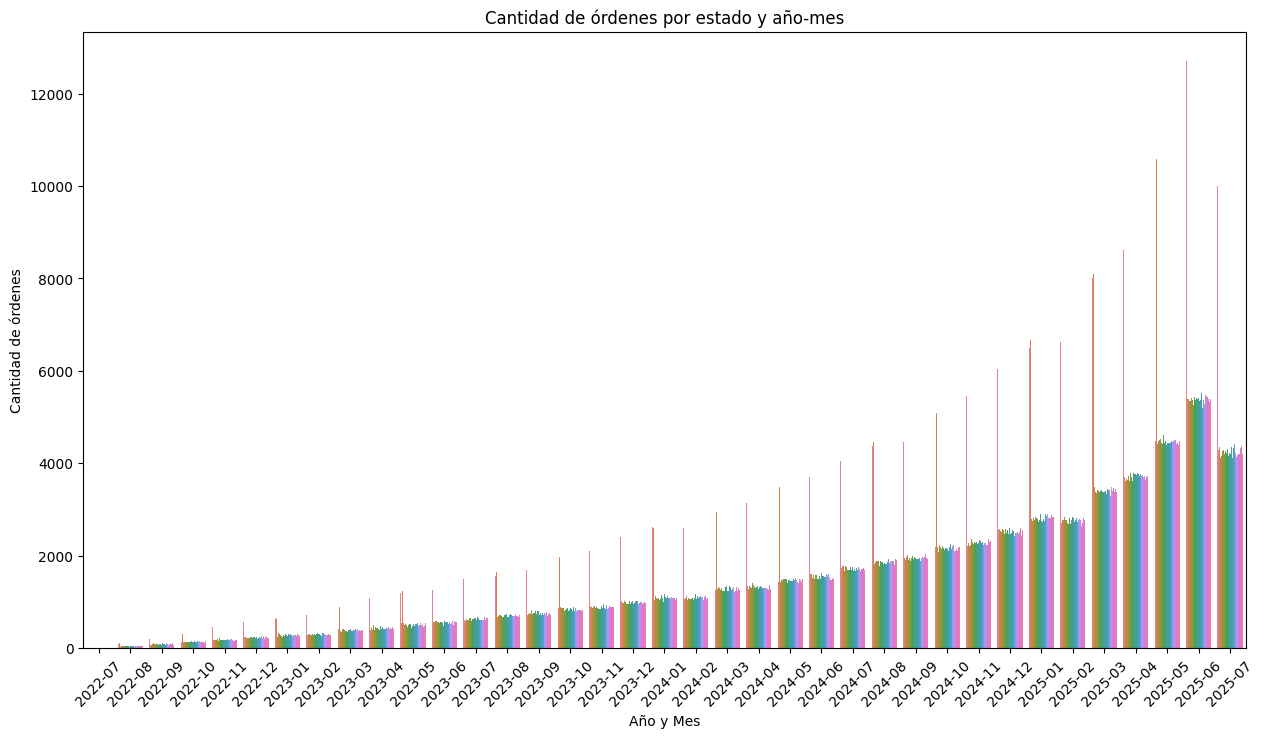
\includegraphics[width=0.8\textwidth]{imagenes/datos_uniformes/ordenes_por_estado_en_el_tiempo.png}
    \caption{Proporción de órdenes por estado en el tiempo}
    \label{fig:ordenes_por_estado_en_el_tiempo}
\end{figure}

La única anomalía en la tendencia que siguen los datos es en el último mes registrado. Esto puede deberse a que los datos fueron generados hasta una fecha específica (17/07/2025) y no se completó el mes, por lo que la cantidad de órdenes en ese mes es considerablemente menor.

\subsection{Inventario}

En la figura \ref{fig:movimientos_por_tipo_y_dia} se puede observar la cantidad de movimientos de inventario por tipo y día. Se puede observar que a lo largo del tiempo se registran cantidades de movimientos similares para cada tipo de movimiento. La única excepción es el tipo de movimiento `Undefined', que tiene una cantidad considerablemente menor de movimientos registrados.

Notar cómo se forman franjas en las cuales se distribuyen los puntos, donde cada uno representa la cantidad de movimientos que hubo en un día. Si los datos fueran reales, se podría esperar ver que las franjas sigan un ciclo anual, con más movimientos en ciertas épocas del año (por ejemplo, en diciembre por las fiestas) y menos en otras. Sin embargo, en este caso las franjas no siguen un patrón anual, sino que parecen estar distribuidas de manera uniforme a lo largo del tiempo.

\begin{figure}[H]
    \centering
    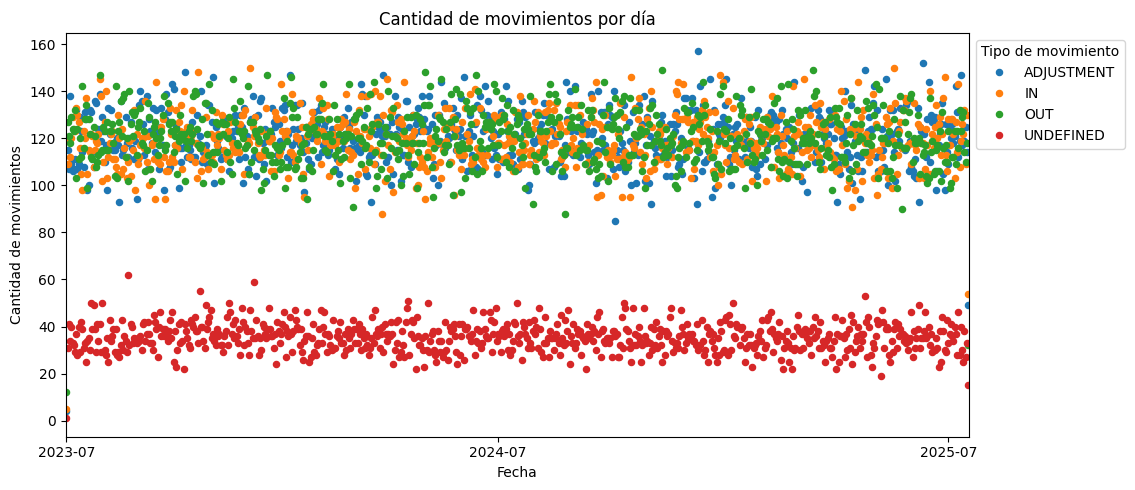
\includegraphics[width=0.8\textwidth]{imagenes/datos_uniformes/movimientos_por_tipo_y_dia.png}
    \caption{Cantidad de movimientos por tipo y día}
    \label{fig:movimientos_por_tipo_y_dia}
\end{figure}

\begin{figure}[H]
    \centering
    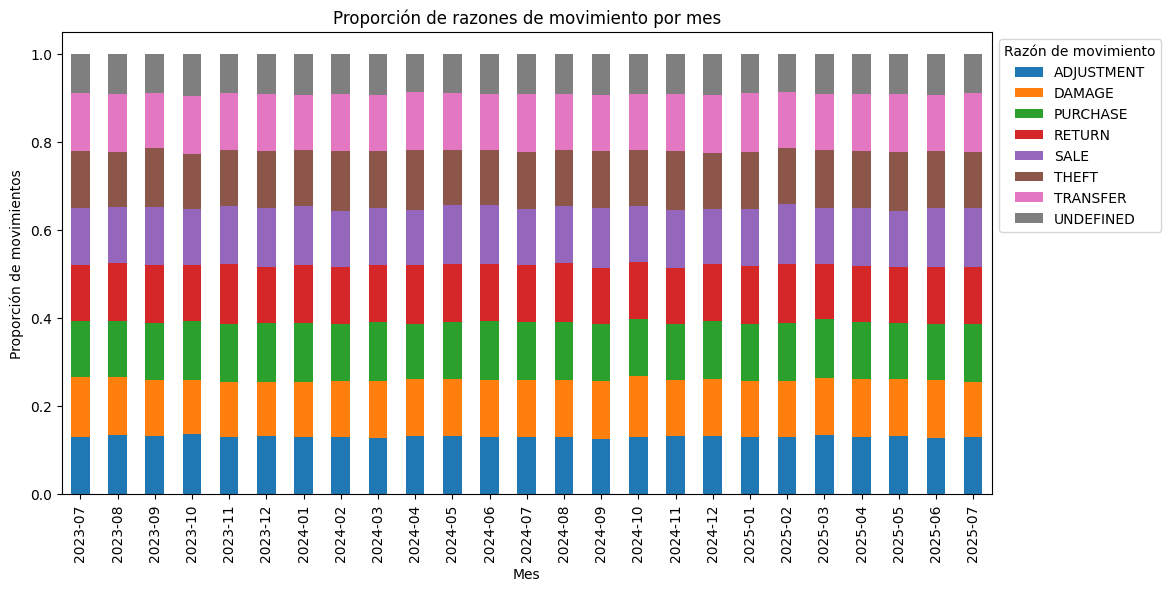
\includegraphics[width=0.8\textwidth]{imagenes/datos_uniformes/razones_de_movimientos.png}
    \caption{Proporción de razones de movimientos por mes}
    \label{fig:razones_de_movimientos}
\end{figure}

En la figura \ref{fig:razones_de_movimientos} nuevamente se puede observar una distribución uniforme en el tiempo, esta vez de las razones de movimientos de inventario. Se puede observar que hay una cantidad muy similar de todos los movimientos, y que la proporción entre ellos se mantiene casi constante a lo largo del tiempo. Por ejemplo podemos ver que la proporción entre movimientos de tipo `Sale' y `Theft' es casi exactamente 1:1 en todos los meses, lo cual sería preocupante en un escenario real.

Finalmente, se presentan dos gráficos que personalmente me gustan mucho. \\
En la figura \ref{fig:cambios_cantidad_mes} se puede observar el cambio acumulado en la cantidad de unidades del inventario (sin diferenciar entre productos). Es notable cómo la línea negra, que representa el cambio total en la cantidad, se mantiene casi constante a lo largo del tiempo, con pequeñas variaciones. Esto indica que la cantidad de unidades en el inventario no varía mucho a lo largo del tiempo. Se puede observar que en todos los meses las cantidades en los movimientos `IN' se compensan con las de los movimientos `OUT', mientras que las cantidades de los movimientos `ADJUSTMENT' y `UNDEFINED' casi no aparecen en el gráfico, lo que indica que las entradas en la tabla se cancelan entre sí en un mismo mes.

Por último, en la figura \ref{fig:distribucion_tipos_de_mov} se puede observar la distribución de los tipos de movimiento en el tiempo. Podemos observar que, aún con una elevada cantidad de \texttt{bins} en el histograma, la distribución de los tipos de movimiento es prácticamente constante para los tipos de movimiento `IN', `OUT' y `ADJUSTMENT'. Además, podemos ver límites muy marcados y redondos en los valores que toma cada tipo de movimiento. \\
También se puede observar que el tipo de movimiento `UNDEFINED' no sigue una distribución uniforme, pero sigue la misma distribución que el total de movimientos. De esta manera podemos inferir que para el dataset se crearon los datos `IN', `OUT' y `ADJUSTMENT' de manera uniforme, y luego los datos `UNDEFINED' se crearon como un porcentaje fijo del total de movimientos.

\begin{figure}[H]
    \centering
    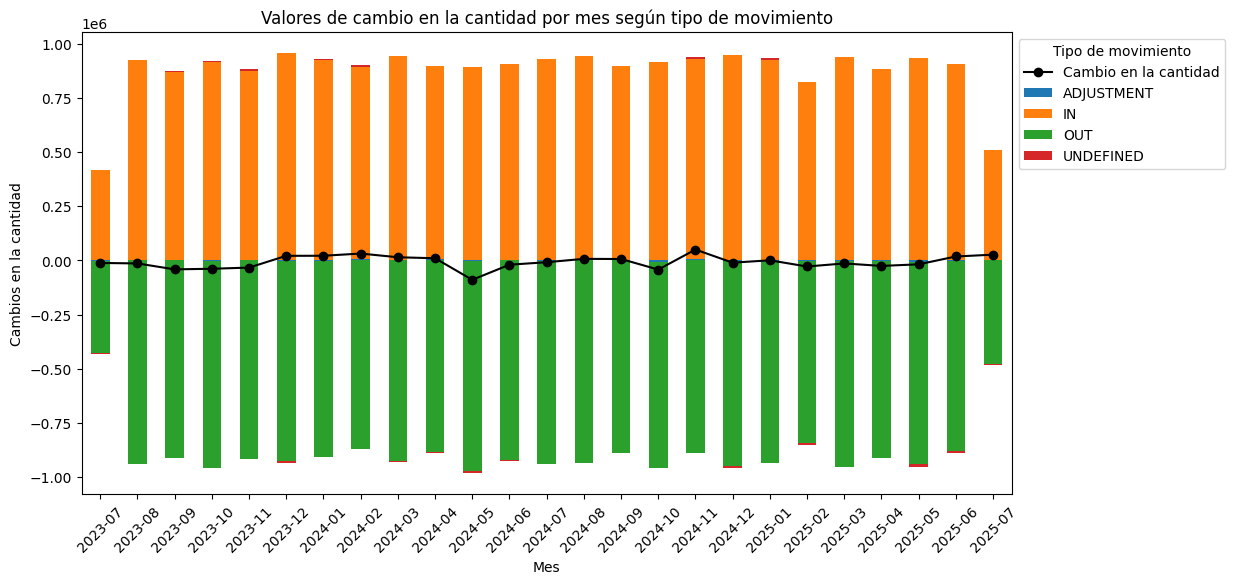
\includegraphics[width=0.8\textwidth]{imagenes/datos_uniformes/cambios_cantidad_mes.png}
    \caption{Valores de cambio en la cantidad por mes según tipo de movimiento}
    \label{fig:cambios_cantidad_mes}
\end{figure}

\begin{figure}[H]
    \centering
    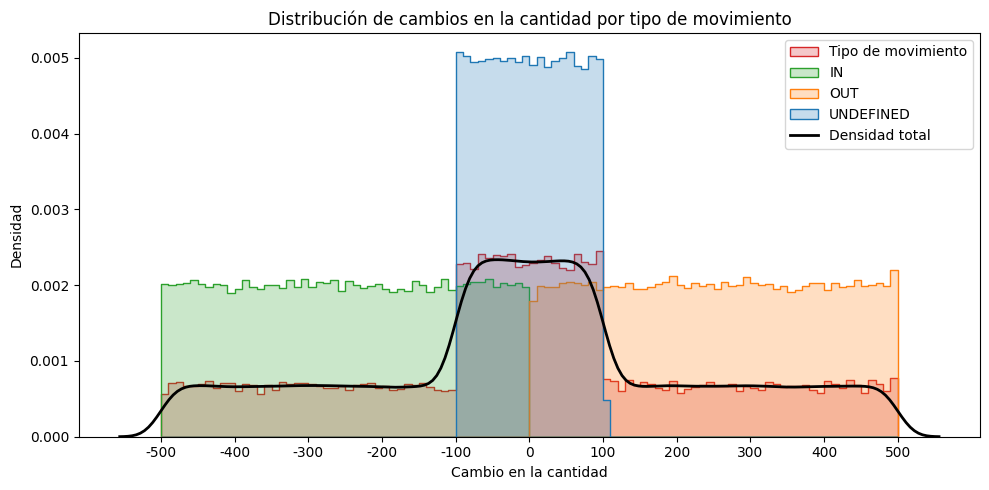
\includegraphics[width=0.8\textwidth]{imagenes/datos_uniformes/distribucion_tipos_de_mov.png}
    \caption{Distribución de valores de cambio en la cantidad según tipo de movimiento}
    \label{fig:distribucion_tipos_de_mov}
\end{figure}

    \section{Consultas y Visualizaciones}
    \subsection{Consultas Propuestas por el Enunciado}

\subsubsection{¿Cuál es el estado que más descuentos tiene en total? ¿y en promedio?}

Para esta consulta se tomaron algunas consideraciones:
\begin{itemize}
    \item Se consideraron los 50 Estados de los Estados Unidos. No se consideraron territorios ni estados militares.
    \item El estado a considerar es el encontrado en la columna \texttt{billing\_address} de la tabla \texttt{orders}.
    \item Se consideraron los "estados con más descuentos" a aquellos que poseen la mayor cantidad de órdenes con descuentos aplicados. Se considera que una orden tiene un descuento si el monto del descuento no es nulo y es mayor a 0.
    \item La segunda parte de la consulta (``¿y en promedio?'') se interpreta como el estado con mayor promedio en el valor de \texttt{discount\_amount}.
\end{itemize}

Para poder realizar esta consulta, fue necesario extraer el estado y el código postal de la columna \texttt{billing\_address} de la tabla \texttt{orders}. 

Las direcciones parecían seguir un patrón que me facilitó extraer el estado y el código postal mediante una expresión regular.
Para esto, primero se normalizaron los datos de la columna y luego se utilizó la siguiente expresión regular:

\begin{lstlisting}[language=Python]
orders["billing_address"] = orders["billing_address"].str.upper()
orders.fillna({"billing_address":"UNDEFINED"}, inplace=True)
pattern = r'([A-Z]{2})\s(\d{5})'
orders[["state", "zip_code"]] = orders["billing_address"].str.extract(pattern)
\end{lstlisting}

La expresión regular extrae dos grupos: el primero corresponde al estado (dos letras mayúsculas) y el segundo al código postal (cinco dígitos).
Para verificar que esta extracción fuera exitosa se realizaron las siguientes comprobaciones, para las cuales se obtuvieron resultados positivos (ver Anexo \ref{anexo:output_validacion_consulta1}).

\begin{lstlisting}[language=Python, xleftmargin=25pt, xrightmargin=25pt, ]
null_state_and_addr = orders["state"].isna() & orders["billing_address"].str.contains("UNDEFINED")

print("Todas las filas que tienen estado nulo, tienen direccion de facturacion indefinida?", 
        "Si" if null_state_and_addr.sum() == orders["state"].isna().sum() else "No")
\end{lstlisting}

Finalmente, para responder la consulta, se creó un filtro que deja fuera los estados militares y territorios llamado \texttt{not\_states\_filter} (ver Anexo \ref{anexo:output_filtro_estados}). Se filtraron las órdenes conservando solo aquellas que tenían un monto de descuento mayor a 0 y que cumplían con el filtro de estados, y se agruparon por estado, contando la cantidad de órdenes con descuento por estado.

\begin{lstlisting}[language=Python, xleftmargin=35pt, xrightmargin=35pt, ]
orders_with_discount = orders.loc[orders["discount_amount"] > 0]
                                .loc[not_states_filter]

quantity_of_orders_with_discounts_by_state = orders_with_discount.groupby("state")["order_id"]
                                                                        .count().reset_index()
\end{lstlisting}

Luego, para visualizar mejor los resultados, se renombraron las columnas y se agregó una columna con el nombre del estado utilizando \texttt{map} (ver Anexo \ref{anexo:output_formateo_resultados}). Se visualizaron los 5 estados con más órdenes utilizando la función \texttt{nlargest} de pandas.

\begin{lstlisting}[language=Python, xleftmargin=35pt, xrightmargin=35pt]
print("\nTop 5 estados con mas ordenes con descuentos:")
quantity_of_orders_with_discounts_by_state.nlargest(5, "Cantidad de Ordenes con Descuento")
\end{lstlisting}
\begin{table}[H]
\centering

\begin{tabular}{|c|c|c|}
\hline
\textbf{Código de Estado} & \textbf{Cantidad de Órdenes con Descuento} & \textbf{Nombre del Estado} \\
\hline
LA & 13,950 & Louisiana \\
MO & 13,940 & Missouri \\
IL & 13,930 & Illinois \\
KY & 13,903 & Kentucky \\
IA & 13,873 & Iowa \\
\hline
\end{tabular}
\caption{Top 5 estados con más órdenes con descuentos}
\end{table}

Entonces la respuesta a ``¿Cuál es el estado que más descuentos tiene en total?'' es Louisiana.

Luego, para encontrar el estado con mayor promedio en el valor de \texttt{discount\_amount}, se calculó el promedio del monto de descuento por estado y se utilizó nuevamente la función \texttt{nlargest} para obtener los 5 estados con mayor promedio.

\begin{lstlisting}[language=Python, xleftmargin=26pt, xrightmargin=26pt]
states_avg_discount = orders_with_discount.groupby("state")["discount_amount"].mean().reset_index()
states_avg_discount.nlargest(5, "discount_amount")
\end{lstlisting}

\begin{table}[H]
\centering
\begin{tabular}{|c|c|c|}
\hline
\textbf{Código de Estado} & \textbf{Promedio de Descuento (\$)} & \textbf{Nombre del Estado} \\
\hline
NC & 50.67 & North Carolina \\
GA & 50.46 & Georgia \\
OK & 50.42 & Oklahoma \\
CO & 50.34 & Colorado \\
MS & 50.32 & Mississippi \\
\hline
\end{tabular}
\caption{Top 5 estados con mayor promedio de monto de descuento}
\end{table}

Entonces la respuesta a ``¿y en promedio?'' es North Carolina.

\subsubsection{¿Cuáles son los 5 códigos postales más comunes para las órdenes con estado `Refunded'? ¿Y cuál es el nombre más frecuente entre los clientes de esas direcciones?}

Para resolver esta consulta, se aprovechó la extracción del código postal realizada sobre la tabla \texttt{orders} en la consulta anterior. 
En primer lugar, se filtraron las órdenes con estado `Refunded` y se contaron la cantidad de órdenes por código postal utilizando la función \texttt{value\_counts}. Luego, se utilizó las función \texttt{nlargest} para obtener los 5 códigos postales más comunes entre las órdenes con estado `Refunded`.

\begin{lstlisting}[language=Python, xleftmargin=35pt, xrightmargin=35pt]
refunded_orders = orders[orders["status"].str.contains("REFUNDED")]

amount_refunded_orders_by_zipcode = refunded_orders["zip_code"].value_counts().reset_index()
top_refunded_zipcodes = amount_refunded_orders_by_zipcode.nlargest(5, "count")

print("\nTop 5 codigos postales mas comunes para ordenes con estado 'Refunded':")
print(top_refunded_zipcodes)
\end{lstlisting}
\begin{table}[H]
\centering
\begin{tabular}{|c|c|}
\hline
\textbf{Código Postal} & \textbf{Cantidad de Órdenes `Refunded`} \\
\hline
31571 & 6 \\
65247 & 5 \\
38151 & 5 \\
09045 & 5 \\
14396 & 5 \\
\hline
\end{tabular}
\caption{Top 5 códigos postales más comunes para órdenes con estado `Refunded`}
\end{table}
Como los puestos 2, 3, 4 y 5 están empatados con 5 órdenes cada uno, se agregó una consulta adicional para ver todos los códigos postales que tienen 5 órdenes `Refunded` (ver Anexo \ref{anexo:output_codigos_postales_refunded}).

Para obtener los nombres más frecuentes entre los clientes de esos códigos postales, se filtró la tabla \texttt{customers} utilizando el método \texttt{isin} para seleccionar únicamente las filas cuyo \texttt{postal\_code} se encuentra en un conjunto específico de valores. Luego se contaron las apariciones de cada nombre utilizando nuevamente la función \texttt{value\_counts}. Para mostrar los 5 nombres más frecuentes, se utilizó la función \texttt{nlargest}.

\begin{lstlisting}[language=Python, xleftmargin=20pt, xrightmargin=20pt]
most_common_names = customers
    .loc[customers["postal_code"].isin(top_refunded_zipcodes["zip_code"])]["first_name"].value_counts()
most_common_names.nlargest(5)
\end{lstlisting}
\begin{table}[H]
\centering
\begin{tabular}{|c|c|}
\hline
\textbf{Nombre} & \textbf{Cantidad de Apariciones} \\
\hline
UNDEFINED & 4 \\
RICHARD & 2 \\
MICHAEL & 2 \\
ROBERT & 1 \\
CYNTHIA & 1 \\
\hline
\end{tabular}
\caption{Top 5 nombres más frecuentes entre los clientes de los códigos postales con más órdenes `Refunded`}
\end{table}

Como puede verse, el nombre más frecuente entre los clientes de esas direcciones es `UNDEFINED`, que aparece 4 veces. Esto significa que hay 4 órdenes registradas por clientes sin nombre registrado. Nuevamente, se realizó una consulta adicional para ver otros nombres que aparecen una sola vez (ver Anexo \ref{anexo:nombres_mas_comunes}).

\subsubsection{Para cada tipo de pago y segmento de cliente, devolver la suma y el promedio expresado como porcentaje, de clientes activos y de consentimiento de marketing.}

Para resolver esta consulta era necesario tener columnas tanto en la tabla \texttt{customers} como en la tabla \texttt{orders}. Por lo tanto, se realizó un \texttt{merge} entre ambas tablas utilizando la columna \texttt{customer\_id} como clave.

\begin{lstlisting}[language=Python, xleftmargin=78pt, xrightmargin=78pt]
orders_customers = orders.merge(customers, on="customer_id").reset_index()
\end{lstlisting}

Luego, para evitar contar dos veces a un mismo cliente que hizo varias órdenes con el mismo método de pago, se eliminaron las filas duplicadas basándose en las columnas \texttt{customer\_id} y \texttt{payment\_method}. 

\begin{lstlisting}[language=Python, xleftmargin=23pt, xrightmargin=23pt]
orders_customers_unique = orders_customers.drop_duplicates(subset=["payment_method", "customer_id"])
\end{lstlisting}

Finalmente, se agrupó por \texttt{payment\_method} y \texttt{customer\_segment}, y se calcularon las funciones de agregación necesarias para obtener la cantidad total de clientes, la cantidad de clientes activos y la cantidad de clientes con consentimiento de marketing. Luego, se calcularon los promedios expresados como porcentaje.

\begin{lstlisting}[language=Python, xleftmargin=100pt, xrightmargin=100pt]
orders_customers_grouped = orders_customers_unique
    .groupby(["payment_method", "customer_segment"]).agg({
        "customer_id": "count",
        "is_active": ["sum", "mean"],
        "marketing_consent": ["sum", "mean"]
    })
orders_customers_grouped[('is_active', 'mean')] *= 100
orders_customers_grouped[('marketing_consent', 'mean')] *= 100
\end{lstlisting}

Me pareció interesante graficar los resultados utilizando un \texttt{heatmap} de la librería \texttt{seaborn}, para lo cual fue necesario reestructurar el DataFrame utilizando la función \texttt{unstack} (ver Anexo \ref{anexo:consulta3_heatmap}). En el notebook también pueden encontrarse los resultados expuestos como tabla.

\subsubsection{Para los productos que contienen en su descripción la palabra `stuff', calcular el peso total de su inventario agrupado por marca}

Para esta consulta, se asumió que la columna \texttt{weight\_kg} representa el peso unitario del producto en el inventario.

Primero se filtraron los productos que contienen la palabra `stuff' en su descripción, sin importar mayúsculas o minúsculas. Para esto se utilizó el método \texttt{str.contains} de pandas, con el parámetro \texttt{case=False} para ignorar mayúsculas y minúsculas. También se seleccionaron únicamente las columnas relevantes para la consulta: \texttt{brand}, \texttt{weight\_kg} y \texttt{stock\_quantity}.

\begin{lstlisting}[language=Python, xleftmargin=0pt, xrightmargin=0pt]
stuff_products = products
    .loc[products["description"].str.contains("STUFF", case=False)][["brand", "weight_kg", "stock_quantity"]]
\end{lstlisting}

Luego, se calculó el peso total de cada producto multiplicando el peso unitario por la cantidad en stock, y se creó una nueva columna llamada \texttt{total\_weight\_kg}. También se eliminaron las columnas que ya no eran necesarias.

\begin{lstlisting}[language=Python, xleftmargin=25pt, xrightmargin=25pt]
stuff_products["total_weight_kg"] = stuff_products["weight_kg"] * stuff_products["stock_quantity"]
stuff_products.drop(columns=["weight_kg", "stock_quantity"], inplace=True)
\end{lstlisting}

Finalmente, se agrupó por marca y se sumó el peso total de los productos de cada marca. Se utilizó la función \texttt{nlargest} para obtener las 5 marcas con mayor peso total en inventario.

\begin{lstlisting}[language=Python, xleftmargin=75pt, xrightmargin=75pt]
    stuff_products.groupby("brand")["total_weight_kg"].sum().nlargest(5)
\end{lstlisting}

\begin{table}[H]
\centering
\begin{tabular}{|c|c|}
\hline
\textbf{Marca} & \textbf{Peso Total (kg)} \\
\hline
UNDEFINED & 11,157,882.66 \\
3M & 2,250,899.67 \\
ADIDAS & 1,923,907.88 \\
NIKE & 1,783,569.90 \\
HASBRO & 1,714,411.24 \\
\hline
\end{tabular}
\caption{Top 5 marcas con mayor peso total de productos con 'stuff' en la descripción}
\end{table}
    
    \subsection{Consultas Propias}
    
    \newpage
    \label{anexo}
\subsection{Output de la Consultas Propuestas por el Enunciado}
Estos outputs pueden encontrarse en el notebook \texttt{propuestas\_del\_enunciado.ipynb}. 
\subsubsection{Consulta 1}
\textbf{Output de la Validación}

\label{anexo:output_validacion_consulta1}
\begin{lstlisting}[style=console]
Filas totales en dataset orders: 4700000
Filas con estado no nulos: 4277862
Filas con estado nulo: 422138
Todas las filas que tienen estado nulo, tienen direccion de facturacion indefinida? Si
\end{lstlisting}

\textbf{Filtro de Estados}

\label{anexo:output_filtro_estados}
\begin{lstlisting}[language=Python]
not_states_filter = ~(
    orders["state"].str.contains("AA")   # Military Americas
    | orders["state"].str.contains("AE") # Military Europe
    | orders["state"].str.contains("AP") # Military Pacific
    | orders["state"].str.contains("FM") # Federated States of Micronesia
    | orders["state"].str.contains("MH") # Marshall Islands
    | orders["state"].str.contains("MP") # Northern Mariana Islands
    | orders["state"].str.contains("PW") # Palau
    | orders["state"].str.contains("GU") # Guam
    | orders["state"].str.contains("VI") # U.S. Virgin Islands
    | orders["state"].str.contains("AS") # American Samoa
    | orders["state"].str.contains("PR") # Puerto Rico
    | orders["state"].str.contains("DC") # District of Columbia
    | orders["state"].isna()             # Nulos
)
print("Cantidad de estados: ", orders.loc[not_states_filter]["state"].unique().size)
print("Estados considerados: ", orders.loc[not_states_filter]["state"].unique())
\end{lstlisting}
\begin{lstlisting}[style=console, aboveskip=0pt]
Cantidad de estados:  50
Estados considerados:  ['ND' 'NJ' 'MN' 'WI' 'OH' 'NV' 'MA' 'AZ' 'MO' 'VT' 'MI' 'NY' 'NM' 'PA'
 'WY' 'NE' 'WV' 'KY' 'WA' 'TX' 'OK' 'ME' 'KS' 'IN' 'FL' 'MD' 'MS' 'AL'
 'MT' 'ID' 'NC' 'AK' 'SD' 'NH' 'SC' 'CT' 'CA' 'CO' 'GA' 'IA' 'VA' 'OR'
 'DE' 'LA' 'UT' 'AR' 'IL' 'TN' 'RI' 'HI']
\end{lstlisting}

\textbf{Formateo de los Resultados}
El archivo json utilizado con los nombres de estado puede encontrarse junto con el código fuente del proyecto.
\label{anexo:output_formateo_resultados}
\begin{lstlisting}[language=Python, xleftmargin=70pt, xrightmargin=70pt]
import json
with open("state_names.json", "r") as f:
    state_names = json.load(f)

quantity_of_orders_with_discounts_by_state["Nombre del Estado"] = 
    quantity_of_orders_with_discounts_by_state["state"].map(state_names)

quantity_of_orders_with_discounts_by_state.rename(
    columns={
        "order_id": "Cantidad de Ordenes con Descuento",
        "state": "Codigo de Estado"
        }, inplace=True
    )
\end{lstlisting}

\subsubsection{Consulta 2}

\textbf{Códigos postales con 5 órdenes `Refunded'}

\label{anexo:output_codigos_postales_refunded}
\begin{lstlisting}[language=Python, xleftmargin=35pt, xrightmargin=35pt]
print("\nCodigos postales con 5 ordenes 'Refunded':")
print(amount_refunded_orders_by_zipcode.loc[amount_refunded_orders_by_zipcode["count"] == 5])
\end{lstlisting}
\begin{lstlisting}[style=console, aboveskip=0pt, xleftmargin=145pt, xrightmargin=145pt]
Codigos postales con 5 ordenes 'Refunded':
   zip_code  count
1     65247      5
2     38151      5
3      9045      5
4     14396      5
5     73291      5
6     91623      5
\end{lstlisting}

\textbf{Otros nombres que aparecen en órdenes `Refunded'}

\label{anexo:nombres_mas_comunes}
\begin{lstlisting}[language=Python, xleftmargin=105pt, xrightmargin=105pt]
print("\nOtros nombres que aparecen una sola vez:")
print(most_common_names.loc[most_common_names == 1].head(7))
\end{lstlisting}
\begin{lstlisting}[style=console, aboveskip=0pt, xleftmargin=145pt, xrightmargin=145pt]
Otros nombres que aparecen una sola vez:
first_name
ROBERT     1
CYNTHIA    1
JAY        1
MARIA      1
KAREN      1
CARLA      1
WILLIAM    1
\end{lstlisting}

\subsubsection{Consulta 3}
\textbf{Gráficos Heatmap resultantes}
\label{anexo:consulta3_heatmap}

\begin{figure}[H]
    \centering
    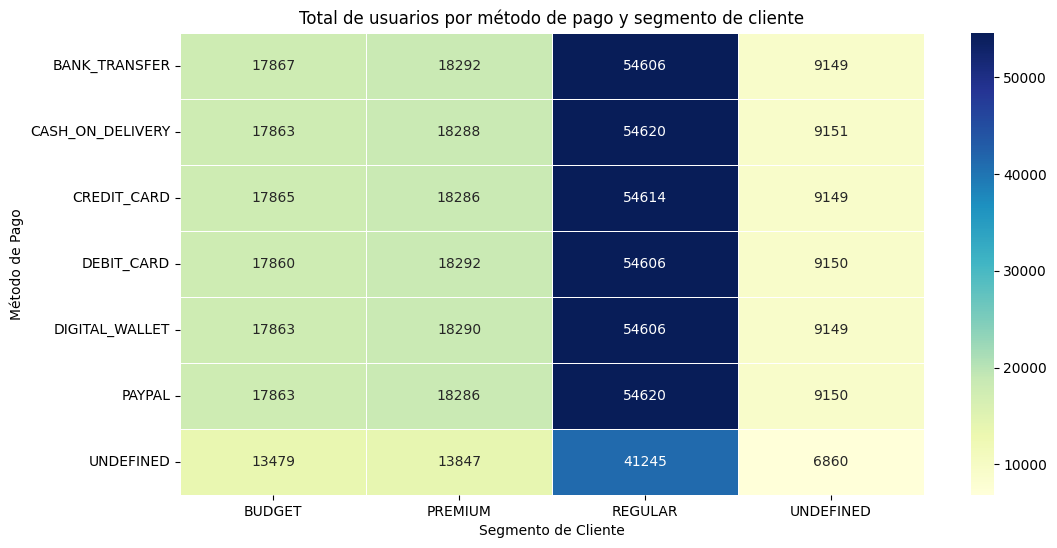
\includegraphics[width=0.8\textwidth]{imagenes/consulta3_heatmap1.png}
\end{figure}

\begin{figure}[H]
    \centering
    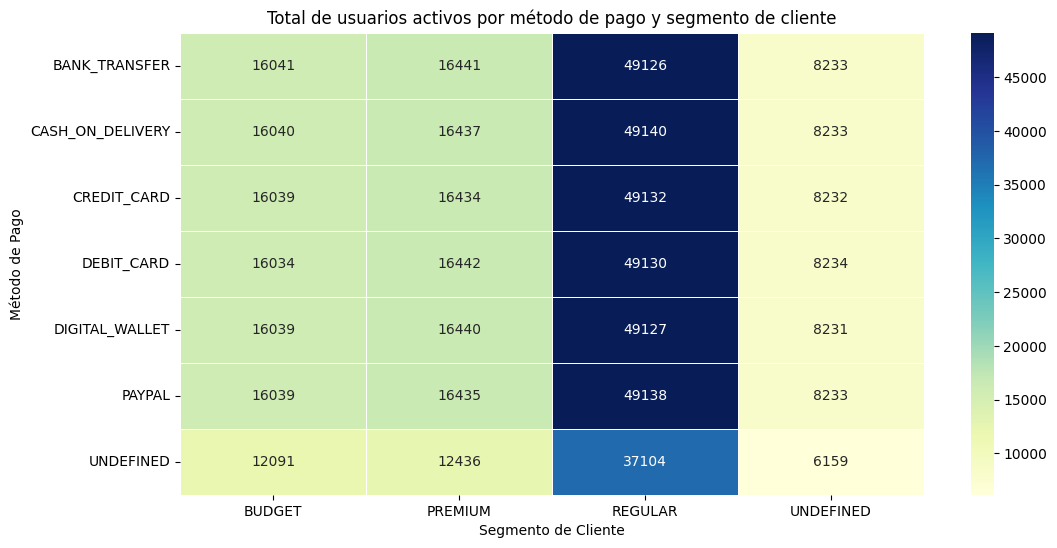
\includegraphics[width=0.8\textwidth]{imagenes/consulta3_heatmap2.png}
\end{figure}

\begin{figure}[H]
    \centering
    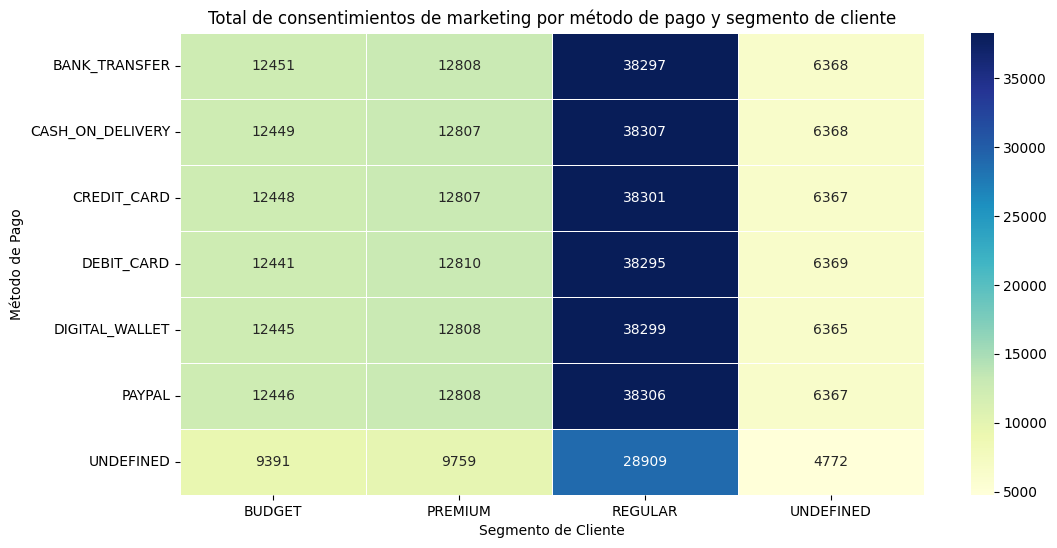
\includegraphics[width=0.8\textwidth]{imagenes/consulta3_heatmap3.png}
\end{figure}

\begin{figure}[H]
    \centering
    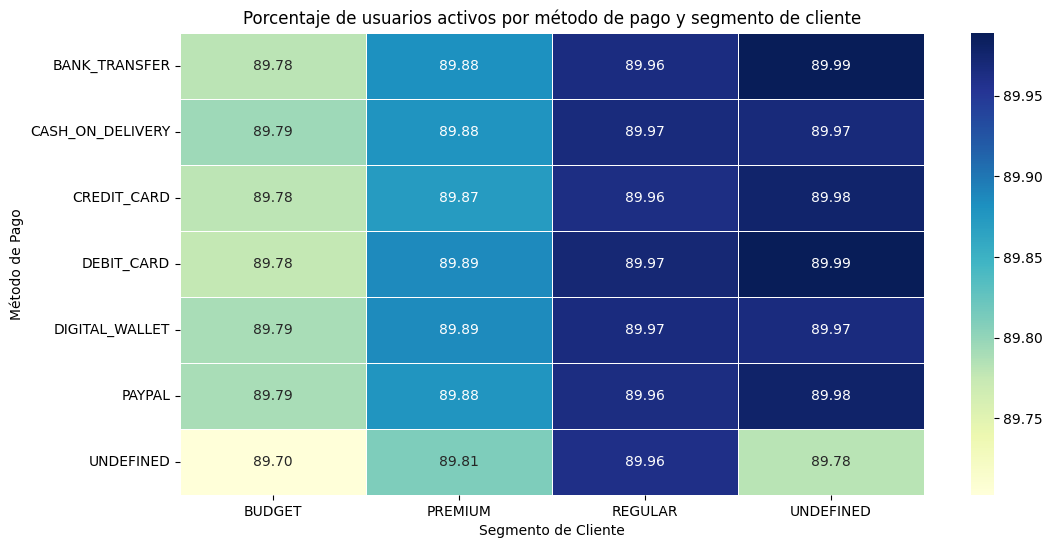
\includegraphics[width=0.8\textwidth]{imagenes/consulta3_heatmap4.png}
\end{figure}

\begin{figure}[H]
    \centering
    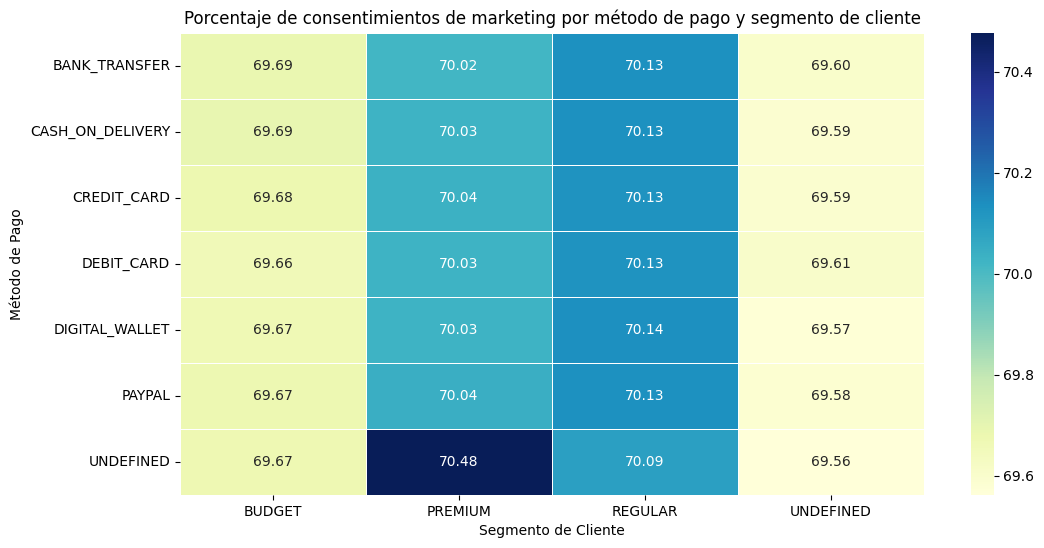
\includegraphics[width=0.8\textwidth]{imagenes/consulta3_heatmap5.png}
\end{figure}
    
\end{document}  